\documentclass[12pt]{article}
\usepackage[T2A]{fontenc}
\usepackage[utf8]{inputenc}
\usepackage[russian]{babel}
\usepackage{geometry}
\usepackage{booktabs}
\usepackage{array}
\usepackage{graphicx}
\usepackage{float}
\usepackage{amsmath}
\usepackage{listings}
\usepackage{xcolor}
\usepackage{hyperref}
\geometry{a4paper, margin=2cm}

\lstset{
  basicstyle=\ttfamily\small,
  breaklines=true,
  frame=single,
  backgroundcolor=\color{gray!10},
  keywordstyle=\color{blue},
  commentstyle=\color{gray},
  stringstyle=\color{teal},
}

\begin{document}

\begin{center}
{\Large Отчёт по лабораторной работе №2}\\[4pt]
{\large Машинное обучение: аппроксимация и классификация}
\end{center}

% ─────────────────────────────────────────────────────────────────────────────
\section{Задание 1. Простые числа и квадратичная аппроксимация (Wolfram Mathematica)}

\subsection{Генерация простых чисел}

Список первых десяти простых чисел сформирован вручную с помощью команд
\texttt{Do}, \texttt{If}, \texttt{IntegerQ}, \texttt{AppendTo} и
\texttt{Complement} без использования встроенных функций поиска простых чисел.
Алгоритм реализует перебор делителей: для каждого кандидата $n$ проверяется,
делится ли он нацело на какое-либо число $k \in [2,\, n{-}1]$ с помощью
\texttt{IntegerQ[n/k]}. Признак простоты определяется через
$\texttt{Complement}[\mathit{divisors},\,\{\}] = \{\}$ — множество делителей
является подмножеством пустого множества только тогда, когда делителей нет.

Полученный список:
\[
  P = \{2,\; 3,\; 5,\; 7,\; 11,\; 13,\; 17,\; 19,\; 23,\; 29\}.
\]

Файлы: \texttt{lab2\_primes.wl} (скрипт), \texttt{lab2\_primes.nb} (блокнот).

\subsection{Аппроксимация по МНК}

По набору точек $\{(i,\, P_i)\}_{i=1}^{10}$ выполнена аппроксимация полиномом
второй степени командой \texttt{Fit[\,points,\,\{1,\,x,\,x\^{}2\},\,x\,]}:
\[
  \hat{f}(x) = 0{,}5667 + 1{,}0227\,x + 0{,}1742\,x^2.
\]

\subsection{Метрики ошибки}

Значения аппроксимирующей функции вычислены с помощью \texttt{Table}; остатки
$e_i = P_i - \hat{f}(i)$ приведены в таблице~\ref{tab:errors}.

\begin{table}[H]
\centering
\caption{Исходные значения, аппроксимация и остатки}
\label{tab:errors}
\begin{tabular}{crrr}
\toprule
$i$ & $P_i$ & $\hat{f}(i)$ & $e_i$ \\
\midrule
1  &  2 &  1{,}764 &  0{,}236 \\
2  &  3 &  3{,}309 & -0{,}309 \\
3  &  5 &  5{,}203 & -0{,}203 \\
4  &  7 &  7{,}445 & -0{,}445 \\
5  & 11 & 10{,}036 &  0{,}964 \\
6  & 13 & 12{,}976 &  0{,}024 \\
7  & 17 & 16{,}264 &  0{,}736 \\
8  & 19 & 19{,}900 & -0{,}900 \\
9  & 23 & 23{,}885 & -0{,}885 \\
10 & 29 & 28{,}218 &  0{,}782 \\
\bottomrule
\end{tabular}
\end{table}

\[
  \text{MSE} = \frac{1}{n}\sum_{i=1}^{n}(P_i - \hat{f}(i))^2 = 0{,}4067,
  \qquad
  \text{MAE} = \frac{1}{n}\sum_{i=1}^{n}|P_i - \hat{f}(i)| = 0{,}5485.
\]
Максимальная абсолютная ошибка равна $0{,}9636$ (при $i=5$, $P_5=11$).

\subsection{Рисунок 1}

На рисунке~\ref{fig:primes} изображены три кривые: ломаная исходных данных
(синий), аппроксимирующая парабола (оранжевый) и кривая модуля ошибки
(красный). Легенды, подписи осей и заголовок сформированы опциями
\texttt{PlotLegends}, \texttt{PlotStyle}, \texttt{Thickness}, \texttt{PlotLabel},
\texttt{AxesLabel}, \texttt{AxesOrigin}.

\begin{figure}[H]
  \centering
  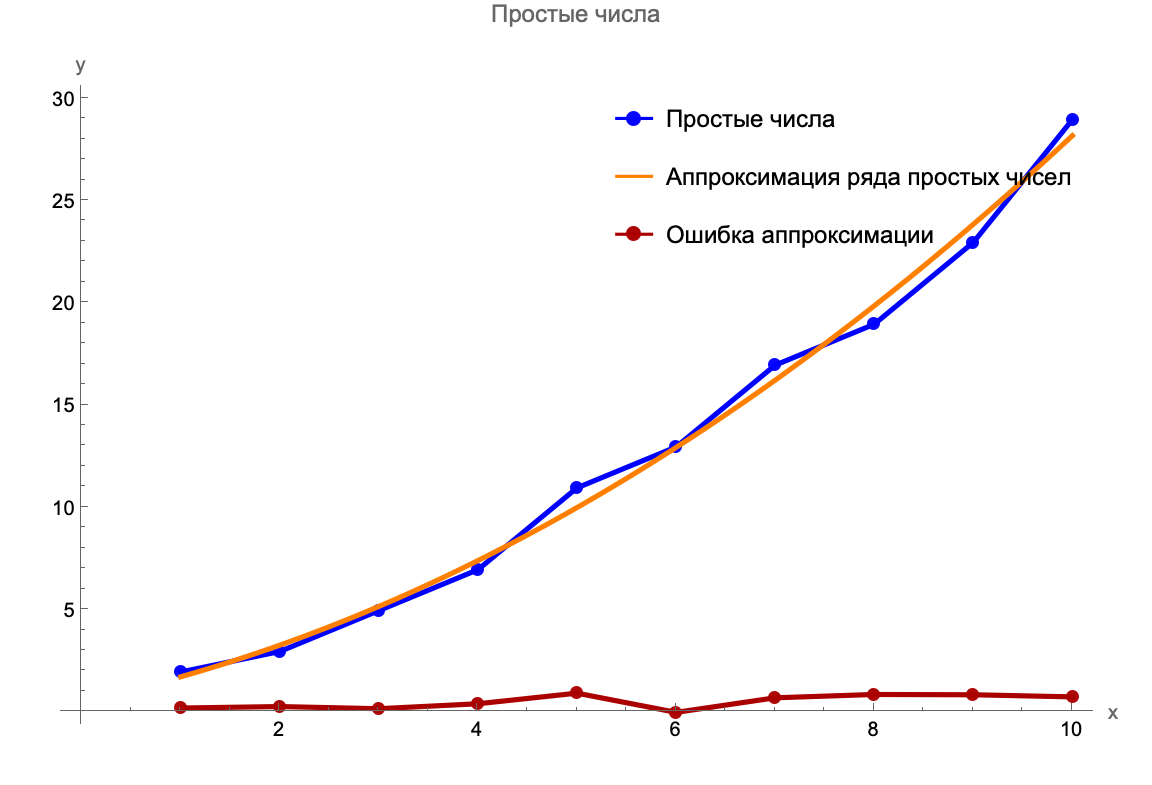
\includegraphics[width=0.78\textwidth]{figure1_with_error.png}
  \caption{Рисунок 1. Простые числа, аппроксимирующая парабола и кривая ошибки}
  \label{fig:primes}
\end{figure}

% ─────────────────────────────────────────────────────────────────────────────
\section{Задание 2. Разметка данных с помощью \texttt{fcluster} (Python)}

\subsection{Исходный набор данных}

В качестве набора данных используются нормированные ответы анкеты из
лабораторной работы~№1 (файл \texttt{../lab1/survey\_normed.csv}).  Анкета
состоит из восьми вопросов (Q1--Q8) о применении AI-инструментов в разработке
программного обеспечения; 100 респондентов, значения нормированы по формуле
min-max в диапазон $[0;\,1]$ с шагом $1/3$.

\subsection{Получение меток кластеров}

Иерархическая кластеризация построена методом Уорда (функция
\texttt{scipy.cluster.hierarchy.linkage}), тем же способом, что и в
лабораторной работе~№1.  Плоская разметка для каждого наблюдения получена
процедурой \texttt{fcluster(Z, t=3, criterion='maxclust')}, разбивающей
дерево на три кластера — в соответствии с уровнем отсечения
$h \approx 3{,}618$, определённым в лабораторной работе~№1.

Распределение по кластерам:
\begin{itemize}
  \item Кластер 1 (консервативные пользователи): 36 наблюдений.
  \item Кластер 2 (активные пользователи AI): 25 наблюдений.
  \item Кластер 3 (прагматичные пользователи): 39 наблюдений.
\end{itemize}

Размечённые данные сохранены в \texttt{lab2\_labeled.csv}.

% ─────────────────────────────────────────────────────────────────────────────
\section{Задание 3. Машинное обучение (Python)}

\subsection{Методология}

На размеченном наборе данных обучены три классификатора:
\begin{itemize}
  \item \textbf{Decision Tree} (дерево решений);
  \item \textbf{Random Forest} (случайный лес);
  \item \textbf{Gradient Boosting Machine, GBM} (градиентный бустинг).
\end{itemize}
Целевая переменная — метка кластера (1, 2 или 3).  Качество оценивалось
стратифицированной 5-кратной перекрёстной проверкой по метрикам
\textbf{accuracy} и \textbf{F1-weighted}.

\subsection{Результаты классификации}

\begin{table}[H]
\centering
\caption{Сравнение классификаторов (5-fold CV, mean ± std)}
\label{tab:models}
\begin{tabular}{lccc}
\toprule
Модель & Accuracy & F1-weighted \\
\midrule
Decision Tree  & $0{,}820 \pm 0{,}068$ & $0{,}814 \pm 0{,}073$ \\
Random Forest  & $\mathbf{0{,}950 \pm 0{,}055}$ & $\mathbf{0{,}950 \pm 0{,}054}$ \\
GBM            & $0{,}920 \pm 0{,}060$ & $0{,}921 \pm 0{,}059$ \\
\bottomrule
\end{tabular}
\end{table}

Наилучший результат по accuracy показал \textbf{Random Forest}
($\text{accuracy} = 0{,}950$, $F1 = 0{,}950$).

\subsection{Внешние параметры лучшей модели — Random Forest}

Внешние (гиперпараметры, задаваемые до обучения) параметры модели Random
Forest, использованной в данной работе:

\begin{table}[H]
\centering
\caption{Гиперпараметры Random Forest}
\label{tab:rf_params}
\begin{tabular}{ll}
\toprule
Параметр & Значение \\
\midrule
\texttt{n\_estimators} (число деревьев) & 200 \\
\texttt{max\_depth} (максимальная глубина дерева) & 5 \\
\texttt{min\_samples\_leaf} (мин. объём листа) & 2 \\
\texttt{criterion} (критерий расщепления) & gini (по умолчанию) \\
\texttt{max\_features} (кол-во признаков на расщепление) & sqrt (по умолчанию) \\
\texttt{bootstrap} (бутстрап выборок) & True (по умолчанию) \\
\texttt{random\_state} (фиксация случайности) & 42 \\
\bottomrule
\end{tabular}
\end{table}

Большое число деревьев (200) снижает дисперсию предсказания и уменьшает риск
переобучения; ограничение глубины (\texttt{max\_depth=5}) дополнительно
регуляризует модель.

\subsection{Анализ информативности переменных}

Информативность переменных оценивалась по встроенному механизму
\texttt{feature\_importances\_} модели Random Forest, основанному на среднем
снижении примеси Джини при использовании каждого признака в качестве
расщепляющего.

\begin{table}[H]
\centering
\caption{Важность признаков (Random Forest, обучение на всём наборе)}
\label{tab:importance}
\begin{tabular}{clrr}
\toprule
Ранг & Признак & Важность & Интерпретация \\
\midrule
1 & Q2 (глубина интеграции AI) & 0{,}243 & \textbf{высокая} \\
2 & Q7 (прирост продуктивности) & 0{,}163 & высокая \\
3 & Q6 (технич.\ интеграция в IDE) & 0{,}146 & высокая \\
4 & Q1 (частота использования AI) & 0{,}133 & средняя \\
5 & Q8 (планы расширения) & 0{,}103 & средняя \\
6 & Q5 (позиция команды) & 0{,}089 & средняя \\
7 & Q3 (уверенность в промптинге) & 0{,}063 & низкая \\
8 & Q4 (доверие к AI-коду) & 0{,}060 & низкая \\
\bottomrule
\end{tabular}
\end{table}

\begin{figure}[H]
  \centering
  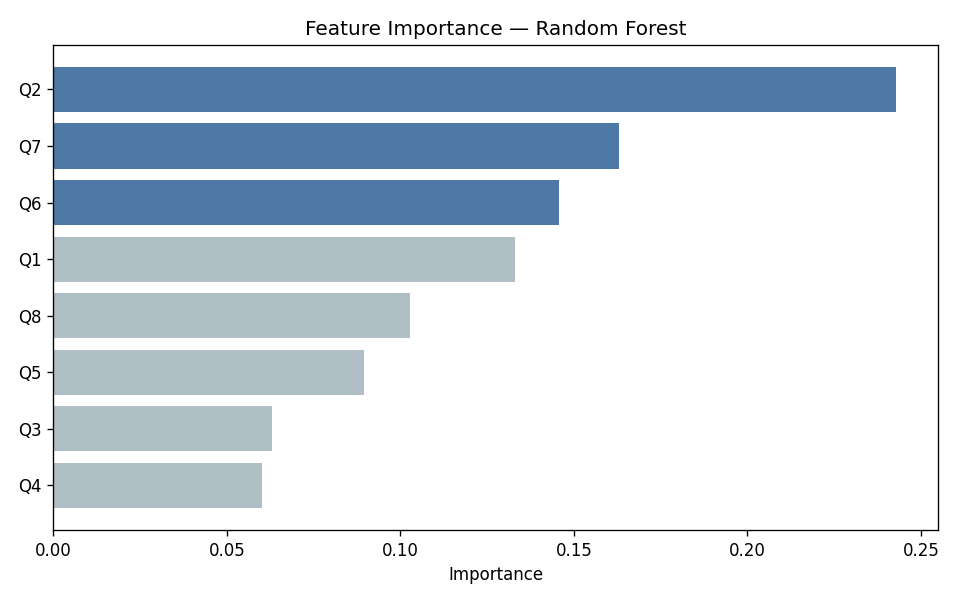
\includegraphics[width=0.75\textwidth]{lab2_feature_importance.png}
  \caption{Важность признаков — Random Forest. Первые три выделены синим.}
  \label{fig:importance}
\end{figure}

\paragraph{Наиболее информативные переменные} (важность $> 0{,}13$):
\begin{itemize}
  \item \textbf{Q2} — глубина интеграции AI в рабочий процесс: наиболее
    значимый признак (0{,}243). Определяет принадлежность к кластеру активных
    пользователей, глубоко встроивших AI в цикл разработки.
  \item \textbf{Q7} — ощущаемый прирост продуктивности (0{,}163): напрямую
    коррелирует с активностью использования AI.
  \item \textbf{Q6} — техническая интеграция в IDE и командные процессы
    (0{,}146): служит маркером «продвинутого» использования, отличающего
    кластер~2 от остальных.
  \item \textbf{Q1} — частота использования (0{,}133): базовый показатель,
    разграничивающий консервативных (кластер~1) и остальных пользователей.
\end{itemize}

\paragraph{Наименее информативные переменные} (важность $< 0{,}07$):
\begin{itemize}
  \item \textbf{Q3} — уверенность в формулировании запросов к AI (0{,}063):
    слабо дифференцирует кластеры, так как различия в навыках промптинга менее
    выражены, чем в глубине интеграции.
  \item \textbf{Q4} — степень доверия к AI-коду после проверки (0{,}060):
    аналогично, данный субъективный показатель менее информативен для
    разграничения групп пользователей.
\end{itemize}

% ─────────────────────────────────────────────────────────────────────────────
\section{Выводы}

\begin{enumerate}
  \item В Wolfram Mathematica список первых 10 простых чисел успешно построен
    с использованием всех требуемых команд (\texttt{Do}, \texttt{If},
    \texttt{IntegerQ}, \texttt{AppendTo}, \texttt{Complement}).
    Квадратичная аппроксимация по МНК даёт приемлемую точность
    ($\text{MSE}=0{,}41$, $\text{MAE}=0{,}55$), максимальное отклонение не
    превышает~1 единицы.

  \item Разметка набора данных из лабораторной работы~№1 с помощью
    \texttt{fcluster} воспроизвела результаты иерархической кластеризации:
    три группы (консервативные, прагматичные, активные пользователи AI)
    размером 36, 39 и 25 наблюдений соответственно.

  \item Лучшей моделью по точности классификации оказался \textbf{Random
    Forest}: $\text{accuracy} = 0{,}950$, $F1 = 0{,}950$ на 5-кратной
    перекрёстной проверке.  Дерево решений (0{,}82) уступает ансамблевым
    методам из-за высокой дисперсии; GBM (0{,}92) занимает промежуточное
    положение.

  \item Анализ информативности признаков выявил четыре ключевые переменные
    (Q2, Q7, Q6, Q1), определяющие принадлежность к кластеру.  Это
    согласуется с выводами лабораторной работы~№1: глубина и частота
    использования AI, техническая интеграция и ощущаемая выгода являются
    главными факторами сегментации разработчиков.  Переменные Q3 и~Q4
    (субъективные оценки навыков и доверия) наименее информативны и при
    необходимости могут быть исключены из модели без существенной потери
    качества.
\end{enumerate}

\end{document}
